\documentclass{standalone}
\usepackage{tikz}
\usepackage{amsmath}

\begin{document}

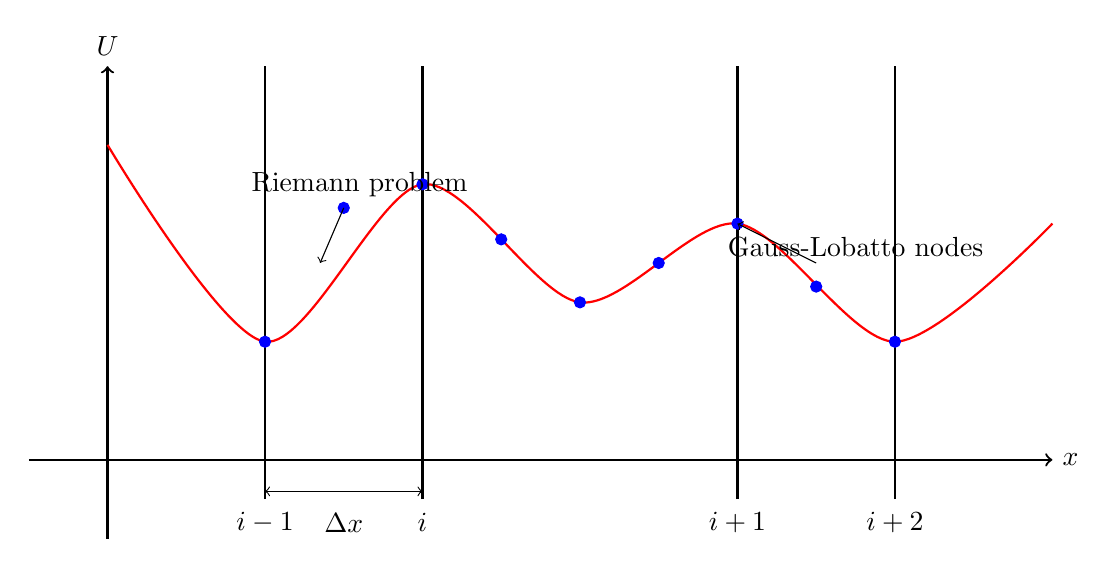
\begin{tikzpicture}

    % Axes
    \draw[thick, ->] (-1, 0) -- (12, 0) node[right] {$x$};
    \draw[thick, ->] (0, -1) -- (0, 5) node[above] {$U$};
    
    % Vertical lines (boundaries)
    \foreach \x in {2, 4, 8, 10} {
        \draw[thick] (\x, -0.5) -- (\x, 5);
    }
    
    % Labels for i-1, i, i+1, etc.
    \node at (2, -0.8) {$i-1$};
    \node at (4, -0.8) {$i$};
    \node at (8, -0.8) {$i+1$};
    \node at (10, -0.8) {$i+2$};
    
    % Curve
    \draw[red, thick] plot [smooth, tension=0.5] coordinates { (0, 4) (2, 1.5) (4, 3.5) (6, 2) (8, 3) (10, 1.5) (12, 3) };
    
    % Gauss-Lobatto nodes (blue dots) - 9 points
    \foreach \x/\y in {2/1.5, 3/3.2, 4/3.5, 5/2.8, 6/2, 7/2.5, 8/3, 9/2.2, 10/1.5} {
        \filldraw[blue] (\x, \y) circle (2pt);
    }
    
    % Riemann problem annotation
    \draw[->] (3, 3.2) -- (2.7, 2.5);
    \node at (3.2, 3.5) {Riemann problem};
    
    % Gauss-Lobatto nodes annotation
    \draw[->] (9, 2.5) -- (8, 3);
    \node at (9.5, 2.7) {Gauss-Lobatto nodes};
    
    % Delta x annotation
    \draw[<->] (2, -0.4) -- (4, -0.4);
    \node at (3, -0.8) {$\Delta x$};
    
\end{tikzpicture}

\end{document}
